\documentclass[12pt]{article}

\usepackage{amsmath}
\usepackage{amsthm}
\usepackage{amssymb}
\usepackage{mathrsfs}
\usepackage{setspace}
\usepackage{graphicx}
\usepackage{caption}
\usepackage{subcaption}
\usepackage{minted}

\newcommand{\w}{\omega}
\renewcommand{\a}{\alpha}
\renewcommand{\d}{\delta}
\newcommand{\s}{\sigma}
\newcommand{\e}{\epsilon}
\newcommand{\m}{\mu}

\newcommand{\inn}[1]{\left\langle #1 \right\rangle}
\newcommand{\norm}[1]{\left\Vert #1 \right\Vert}
\newcommand{\abs}[1]{\left\vert #1 \right\vert}

\newcommand{\real}{\mathbb{R}}
\newcommand{\nat}{\mathbb{Z}^+}

\begin{document}

\title{Homework 6}
\date{\today}
\author{Hunter Schwartz}
\maketitle

%\doublespacing

\textbf{Problem 1}

(a) We have

\begin{align*}
&y(h) = y(0) + hy'(0) + \frac{h^2}{2}y''(0) + \frac{h^3}{6}y'''(0) + O(h^4), \\
\implies& y''(0) = \frac{2}{h^2} y(h) - \frac{2}{h^2}y(0) - \frac{2}{h}y'(0) - \frac{h}{3}y'''(0) + O(h^2).
\end{align*}

Also,

\begin{align*}
&y(2h) = y(0) + 2hy'(0) + 2h^2 y''(0) + \frac{4h^3}{3}y'''(0) + O(h^4), \\
\implies& y''(0) = \frac{1}{2h^2}y(2h) - \frac{1}{2h^2}y(0) - \frac{1}{h}y'(0) - \frac{2h}{3}y'''(0) + O(h^2).
\end{align*}

We want to choose $c_1,c_2$ such that a combination of these representations is $O(h^2)$:

\begin{align*}
y''(0) &= c_1y''(0) + c_2y''(0) \\
&= c_2\frac{1}{2h^2}y(2h) + c_1 \frac{2}{h^2} y(h) - (c_1\frac{2}{h^2} + c_2\frac{1}{2h^2})y(0) - (c_1\frac{2}{h} + c_2\frac{1}{h})y'(0) \\
&\quad\quad - (c_1\frac{h}{3} + c_2\frac{2h}{3})y'''(0) + O(h^2) \\
&= c_2\frac{1}{2h^2}y(2h) + c_1 \frac{2}{h^2} y(h) - (c_1\frac{2}{h^2} + c_2\frac{1}{2h^2})y(0) + O(h^2).
\end{align*}

Therefore, we need to satisfy the system of equations

\begin{align*}
c_1 + c_2 &= 1, \\
2c_1 + c_2 &= 0, \\
c_1 + 2c_2 &= 0.
\end{align*}

These three equations cannot be simultaneously satisfied by any choice of $c_1,c_2$, so there is no way to approximate $y''(0)$ to the desired order with the given values.

\newpage

(b) We know

\begin{align*}
&y(3h) = y(0) + 3hy'(0) + \frac{9h^2}{2}y''(0) + \frac{9h^3}{2}y'''(0) + O(h^4), \\
\implies& y''(0) = \frac{2}{9h^2} y(3h) - \frac{2}{9h^2}y(0) - \frac{2}{3h}y'(0) - hy'''(0) + O(h^2).
\end{align*}

Including the results of part (a), we have

\begin{align*}
y''(0) &= \frac{2}{h^2} y(h) - \frac{2}{h^2}y(0) - \frac{2}{h}y'(0) - \frac{h}{3}y'''(0) + O(h^2), \\
&= \frac{1}{2h^2}y(2h) - \frac{1}{2h^2}y(0) - \frac{1}{h}y'(0) - \frac{2h}{3}y'''(0) + O(h^2), \\
&= \frac{2}{9h^2} y(3h) - \frac{2}{9h^2}y(0) - \frac{2}{3h}y'(0) - hy'''(0) + O(h^2).
\end{align*}

For the desired accuracy, we need to choose $c_1,c_2,c_3$ such that

\begin{align*}
y''(0) &= c_1y''(0) + c_2y''(0) + c_3y''(0) \\
&= c_3\frac{2}{9h^2} y(3h) + c_2\frac{1}{2h^2}y(2h) + c_1 \frac{2}{h^2} y(h) - (c_1\frac{2}{h^2} + c_2\frac{1}{2h^2} + c_3\frac{2}{9h^2})y(0) \\
&\quad\quad - (c_1\frac{2}{h} + c_2\frac{1}{h} + c_3\frac{2}{3h})y'(0) - (c_1\frac{h}{3} + c_2\frac{2h}{3} + c_3h)y'''(0) + O(h^2) \\
&= c_3\frac{2}{9h^2} y(3h) + c_2\frac{1}{2h^2}y(2h) + c_1 \frac{2}{h^2} y(h) - (c_1\frac{2}{h^2} + c_2\frac{1}{2h^2} + c_3\frac{2}{9h^2})y(0) + O(h^2).
\end{align*}

Thus, we need to satisfy the system of equations

\begin{align*}
c_1 + c_2 + c_3 = 1, \\
2c_1 + c_2 + \frac{2}{3}c_3 = 0, \\
\frac{1}{3}c_1 + \frac{2}{3}c_2 + c_3 = 0.
\end{align*}

This system is solved by $c_1 = -\frac{5}{2}, c_2 = 8, c_3 = -\frac{9}{2}$.

Substituting these values into the equation for $y''(0)$ and simplifying, we find

\begin{align*}
y''(0) = \frac{2y(0) - 5y(h) + 4y(2h) - y(3h)}{h^2} + O(h^2).
\end{align*}

\newpage

\textbf{Problem 2}

We want to solve $-(y')' + (\frac{\pi}{2})^2 = x$ on $(0,1)$ with $y(0) = y(1) = 0$. Given our basis $\{\sin(n\pi x)\}_{n=1}^N$, this reduces to solving the equation $Ax = b$ for $x$, with 

\begin{align*}
(A)_{ij} &= \int_0^1 [\sin(i\pi x)]'\cdot[\sin(j\pi x)]'dx + \int_0^1 \left(\frac{\pi}{2}\right)^2 \sin(i\pi x) \sin(j\pi x) dx \\
&= ij\pi^2 \int_0^1 \cos(i\pi x) \cos(j\pi x)dx + \left(\frac{\pi}{2}\right)^2 \int_0^1 \sin(i\pi x) \sin(j\pi x) dx, \\
(b)_i &= \int_0^1 x\sin(i\pi x) dx.
\end{align*}

The basis functions are orthogonal on this interval, and we know that $\int_0^1 \sin(i\pi x) \sin(j\pi x) dx = \frac{1}{2} \d_{ij}$. Similarly, $\int_0^1 \cos(i\pi x) \cos(j\pi x) dx = \frac{1}{2} \d_{ij}$. Also, we find that $\int_0^1 x\sin(i\pi x) = \frac{(-1)^{i-1}}{i\pi}$. Thus, $A$ and $b$ are such that

\begin{align*}
(A)_{ij} &= \frac{\pi^2}{8}(4i^2 + 1)\d_{ij}, \\
(b)_i &= \frac{(-1)^{i-1}}{i\pi}.
\end{align*}

We construct the Galerkin method with $N=2$ like so, with the results following.

\begin{minted}{python}
import numpy as np

# domain
x0 = 0
x1 = 1
qsize = 100  # ~quarter of grid size
size = 4*qsize + 1  # ensures can calculate error at desired points
x = np.linspace(x0,x1,size)

# exact solution
def exact(x):
    return -4/(np.pi**2)/np.sinh(np.pi/2) * np.sinh(np.pi/2*x) + 4/(np.pi**2)*x

# generic basis function
def phi(n,x):
    return np.sin(n*np.pi*x)

# setup Galerkin method
N = 2
A = np.diag( [(4*(i+1)**2 + 1) * np.pi**2/8 for i in range(N)] )
b = [(-1)**i / (i+1) / np.pi for i in range(N)]

# solve for coefficient of basis functions
a = np.linalg.solve(A,b)

# Galerkin approximation
y = np.zeros_like(x)
for i in range(N):
    y += a[i]*phi(i+1,x)
\end{minted}

\begin{figure}[h]
\centering
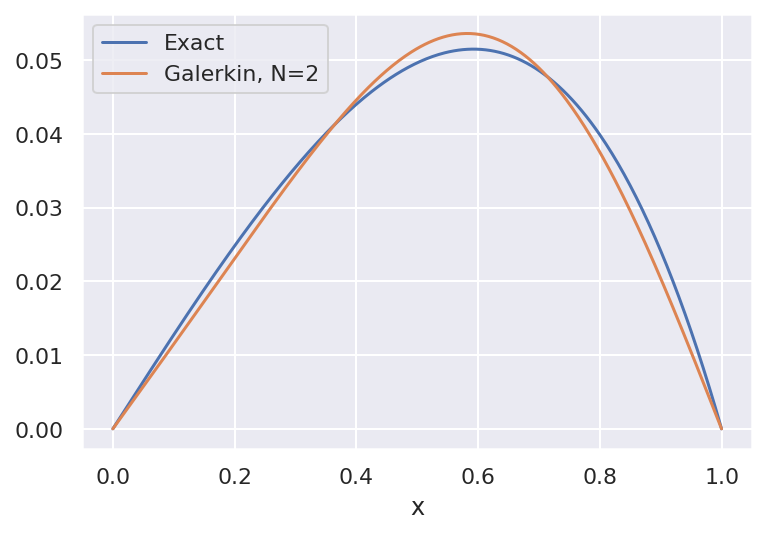
\includegraphics[width=.75\textwidth]{plt.png}
\caption{Comparison of the exact solution to the system vs the approximation due to the Galerkin method, with 2 basis functions.}
\end{figure}

In the end, we find that $c_1 = 0.05160246$ and $c_2 = -0.0075886$. We also have the following data, with $Y(x)$ the exact solution and $y(x)$ the Galerkin approximation:

\begin{center}
\begin{tabular}{ c | c | c }
 $x$ & $y(x) - Y(x)$ & $\frac{y(x) - Y(x)}{Y(x)}$ \\ \hline
 .25 & -0.0014713 & -0.0484442 \\  
 .5  &  0.0019428 &  0.0391235 \\
 .75 & -0.0009743 & -0.0216283
\end{tabular}
\end{center}

\end{document}